% ============================================================
%  Fake News Detection -- Industrial Grade
%  LaTeX Beamer Presentation  |  Internship @ Elevvo
%  Author: Abdullah Zahid
%
%  Compile with:  pdflatex fake_news_presentation.tex  (x2)
%  Requirements:  texlive-latex-extra, texlive-science,
%                 texlive-fonts-recommended, pgfplots, tcolorbox
% ============================================================
\documentclass[aspectratio=169,10pt]{beamer}

\usepackage[T1]{fontenc}
\usepackage[utf8]{inputenc}
\usepackage{helvet}
\renewcommand{\familydefault}{\sfdefault}
\usepackage{xcolor}
\usepackage{tikz}
\usetikzlibrary{shapes.geometric,arrows.meta,positioning,calc}
\usepackage{pgfplots}
\pgfplotsset{compat=1.18}
\usepackage{booktabs}
\usepackage{array}
\usepackage{colortbl}
\usepackage{tabularx}
\usepackage{tcolorbox}
\tcbuselibrary{skins,breakable}
\usepackage{amsmath}

% ── Colour palette ───────────────────────────────────────────
\definecolor{NavyDark}{HTML}{0F172A}
\definecolor{NavyMid}{HTML}{1E293B}
\definecolor{Navy}{HTML}{1B3A6B}
\definecolor{NavyML}{HTML}{2C5282}
\definecolor{ABlue}{HTML}{3B82F6}
\definecolor{BlueL}{HTML}{DBEAFE}
\definecolor{BlueMid}{HTML}{BFDBFE}
\definecolor{Slate}{HTML}{64748B}
\definecolor{SlateL}{HTML}{F1F5F9}
\definecolor{ARed}{HTML}{EF4444}
\definecolor{RedL}{HTML}{FEE2E2}
\definecolor{AGreen}{HTML}{16A34A}
\definecolor{GreenL}{HTML}{DCFCE7}
\definecolor{AOrange}{HTML}{F59E0B}
\definecolor{OrangeL}{HTML}{FEF3C7}
\definecolor{APurple}{HTML}{7C3AED}
\definecolor{PurpleL}{HTML}{EDE9FE}
\definecolor{ATeal}{HTML}{0891B2}
\definecolor{TealL}{HTML}{CFFAFE}
\definecolor{CodeBg}{HTML}{1E293B}
\definecolor{CodeBlue}{HTML}{7DD3FC}
\definecolor{CodeGray}{HTML}{94A3B8}
\definecolor{Gold}{HTML}{F59E0B}

% ── Beamer theme ─────────────────────────────────────────────
\usetheme{default}
\usecolortheme{default}
\setbeamertemplate{navigation symbols}{}
\setbeamertemplate{footline}{}
\setbeamertemplate{headline}{}
\setbeamercolor{background canvas}{bg=SlateL}
\setbeamercolor{frametitle}{bg=Navy,fg=white}
\setbeamerfont{frametitle}{size=\large,series=\bfseries}

\setbeamertemplate{frametitle}{%
  \nointerlineskip
  \begin{beamercolorbox}[wd=\paperwidth,ht=0.95cm,dp=0.20cm,leftskip=0.4cm]{frametitle}%
    \vbox to 0.85cm{%
      \vfill
    \usebeamerfont{frametitle}\insertframetitle
    \ifx\insertframesubtitle\empty\else
      \\[-1pt]{\scriptsize\color{Slate}\itshape\insertframesubtitle}\fi
    \vfill}%
  \end{beamercolorbox}%
  }

% ── Footer macro ─────────────────────────────────────────────
\newcommand{\sfooter}{%
  \begin{tikzpicture}[remember picture,overlay]
    \fill[NavyMid](current page.south west) rectangle ++(\paperwidth,.33cm);
    \node[anchor=west,font=\tiny,text=Slate] at
      ([xshift=.3cm,yshift=.165cm]current page.south west)
      {Elevvo Internship\ \textbullet\ Fake News Detection\ \textbullet\ Abdullah Zahid};
    \node[anchor=east,font=\tiny,text=Slate] at
      ([xshift=-.3cm,yshift=.165cm]current page.south east)
      {\insertframenumber/\inserttotalframenumber};
  \end{tikzpicture}}

% ── tcolorbox styles ─────────────────────────────────────────
\tcbset{
  mycard/.style 2 args={
    colback=white,colframe=#1,boxrule=0.8pt,arc=2pt,
    left=5pt,right=5pt,top=4pt,bottom=4pt,
    drop shadow={opacity=0.07,color=#2}},
  statbox/.style={
    colframe=#1,colback=#1,boxrule=0pt,arc=2pt,
    halign=center,left=4pt,right=4pt,top=5pt,bottom=5pt},
  codeblock/.style={
    colback=CodeBg,colframe=Navy,boxrule=0.7pt,arc=2pt,
    left=6pt,right=6pt,top=5pt,bottom=5pt,
    fontupper=\ttfamily\scriptsize\color{CodeBlue}},
  sideline/.style={
    colback=white,colframe=#1,boxrule=0pt,
    borderline west={3pt}{0pt}{#1},arc=0pt,
    left=6pt,right=4pt,top=2pt,bottom=2pt}
}

% ── pgfplots style ───────────────────────────────────────────
\pgfplotsset{
  indbar/.style={
    ybar,bar width=13pt,enlarge x limits=0.25,
    axis x line=none,axis y line=left,
    y axis line style={draw=none},tick style={draw=none},
    ymajorgrids,grid style={color=BlueMid,line width=0.3pt},
    x tick label style={font=\tiny,color=Slate,rotate=18,anchor=north east},
    y tick label style={font=\tiny,color=Slate},
    nodes near coords,
    every node near coord/.append style={font=\tiny\bfseries,color=white,yshift=1pt},
    clip=false}}

%=============================================================
\newcommand{\pbox}[4]{%
  \fill[#1](#2,0) rectangle ++(2.5,.36);
  \draw[#1,line width=.7pt](#2,-1.6) rectangle ++(2.5,1.6);
  \node[font=\tiny\bfseries,text=white,anchor=center] at (#2+1.25,.18){#3};
  \node[font=\tiny,text=Slate,text width=2.2cm,align=center] at (#2+1.25,-0.78){#4};}

\begin{document}

%------------------------------------------------------------
% SLIDE 1: TITLE
%------------------------------------------------------------
{\setbeamercolor{background canvas}{bg=NavyDark}
\begin{frame}[plain]
\begin{tikzpicture}[remember picture,overlay]
  \fill[NavyML,opacity=.35]
    ([xshift=-2.2cm,yshift=.8cm]current page.north east) circle(2cm);
  \fill[ABlue,opacity=.20]
    ([xshift=-1.4cm,yshift=-.5cm]current page.north east) circle(1.4cm);
  \fill[ABlue](current page.north west) rectangle ++(.11,-\paperheight);
  \fill[ABlue]
    ([xshift=.55cm,yshift=-1.05cm]current page.north west) rectangle ++(2.3cm,.32cm);
  \node[anchor=west,font=\tiny\bfseries,text=white] at
    ([xshift=.62cm,yshift=-.89cm]current page.north west){INTERNSHIP PROJECT};
  \node[anchor=north west,
    font=\fontsize{36}{40}\bfseries\selectfont,text=white,text width=12cm] at
    ([xshift=.55cm,yshift=-1.42cm]current page.north west){Fake News};
  \node[anchor=north west,
    font=\fontsize{36}{40}\bfseries\selectfont,text=ABlue,text width=12cm] at
    ([xshift=.55cm,yshift=-2.82cm]current page.north west){Detection System};
  \node[anchor=north west,font=\small\itshape,text=Slate,text width=11cm] at
    ([xshift=.55cm,yshift=-4.0cm]current page.north west)
    {Industrial-Grade NLP \& Machine Learning Pipeline};
  \draw[ABlue,line width=1.2pt]
    ([xshift=.55cm,yshift=-4.45cm]current page.north west) -- ++(5.5cm,0);
  \node[anchor=north west,font=\scriptsize,text=Slate] at
    ([xshift=.55cm,yshift=-4.7cm]current page.north west){Author};
  \node[anchor=north west,font=\small\bfseries,text=white] at
    ([xshift=.55cm,yshift=-5.0cm]current page.north west){Abdullah Zahid};
  \node[anchor=north west,font=\scriptsize,text=Slate] at
    ([xshift=4.4cm,yshift=-4.7cm]current page.north west){Internship};
  \node[anchor=north west,font=\small\bfseries,text=white] at
    ([xshift=4.4cm,yshift=-5.0cm]current page.north west){Elevvo};
  \node[anchor=north west,font=\scriptsize,text=Slate] at
    ([xshift=7.8cm,yshift=-4.7cm]current page.north west){Task};
  \node[anchor=north west,font=\small\bfseries,text=white,text width=6cm] at
    ([xshift=7.8cm,yshift=-5.0cm]current page.north west)
    {Task 3 --- Binary NLP Classification};
  \fill[NavyMid](current page.south west) rectangle ++(\paperwidth,.38cm);
  \node[anchor=west,font=\tiny,text=Slate] at
    ([xshift=.3cm,yshift=.19cm]current page.south west)
    {Elevvo Internship Program\ \textbullet\ Fake News Detection\ \textbullet\ NLP \& ML};
\end{tikzpicture}
\end{frame}}

%------------------------------------------------------------
% SLIDE 2: TABLE OF CONTENTS
%------------------------------------------------------------
\begin{frame}[t]
\frametitle{Table of Contents}
\framesubtitle{Project overview --- 12 structured steps}
\vspace{.12cm}
\begin{columns}[t]
\begin{column}{.48\textwidth}
\vspace{-15pt}
  \begin{tcolorbox}[mycard={ABlue}{ABlue},borderline west={4pt}{0pt}{ABlue},top=2pt,bottom=2pt]
    \textcolor{ABlue}{\textbf{01}}\quad\textbf{\small Project Overview \& Objectives}\\
    {\tiny\color{Slate}Dataset, goals, and industrial features}
  \end{tcolorbox}\vspace{1pt}
  \begin{tcolorbox}[mycard={ATeal}{ATeal},borderline west={4pt}{0pt}{ATeal},top=2pt,bottom=2pt]
    \textcolor{ATeal}{\textbf{02}}\quad\textbf{\small Dataset \& EDA}\\
    {\tiny\color{Slate}44,000+ articles, class balance, analysis}
  \end{tcolorbox}\vspace{1pt}
  \begin{tcolorbox}[mycard={AGreen}{AGreen},borderline west={4pt}{0pt}{AGreen},top=2pt,bottom=2pt]
    \textcolor{AGreen}{\textbf{03}}\quad\textbf{\small Text Preprocessing Pipeline}\\
    {\tiny\color{Slate}Stopwords, lemmatization, OOP class}
  \end{tcolorbox}\vspace{1pt}
  \begin{tcolorbox}[mycard={AOrange}{AOrange},borderline west={4pt}{0pt}{AOrange},top=2pt,bottom=2pt]
    \textcolor{AOrange}{\textbf{04}}\quad\textbf{\small TF-IDF Feature Engineering}\\
    {\tiny\color{Slate}Bigrams, 50k features, sublinear TF}
  \end{tcolorbox}\vspace{1pt}
  \begin{tcolorbox}[mycard={APurple}{APurple},borderline west={4pt}{0pt}{APurple},top=2pt,bottom=2pt]
    \textcolor{APurple}{\textbf{05}}\quad\textbf{\small Model Training \& Comparison}\\
    {\tiny\color{Slate}4 classifiers + 5-Fold Cross-Validation}
  \end{tcolorbox}
\end{column}
\begin{column}{.48\textwidth}
\vspace{-15pt}
  \begin{tcolorbox}[mycard={Navy}{Navy},borderline west={4pt}{0pt}{Navy},top=2pt,bottom=2pt]
    \textcolor{Navy}{\textbf{06}}\quad\textbf{\small Ensemble Voting Classifier}\\
    {\tiny\color{Slate}Soft voting --- LR + SVC + Naive Bayes}
  \end{tcolorbox}\vspace{1pt}
  \begin{tcolorbox}[mycard={ARed}{ARed},borderline west={4pt}{0pt}{ARed},top=2pt,bottom=2pt]
    \textcolor{ARed}{\textbf{07}}\quad\textbf{\small Evaluation Dashboard}\\
    {\tiny\color{Slate}Accuracy, F1, ROC-AUC, PR Curve}
  \end{tcolorbox}\vspace{1pt}
  \begin{tcolorbox}[mycard={ATeal}{ATeal},borderline west={4pt}{0pt}{ATeal},top=2pt,bottom=2pt]
    \textcolor{ATeal}{\textbf{08}}\quad\textbf{\small Explainability \& Word Clouds}\\
    {\tiny\color{Slate}Feature importance + visual insights}
  \end{tcolorbox}\vspace{1pt}
  \begin{tcolorbox}[mycard={AGreen}{AGreen},borderline west={4pt}{0pt}{AGreen},top=2pt,bottom=2pt]
    \textcolor{AGreen}{\textbf{09}}\quad\textbf{\small Production Deployment}\\
    {\tiny\color{Slate}Model persistence, inference function}
  \end{tcolorbox}\vspace{1pt}
  \begin{tcolorbox}[mycard={Gold}{Gold},borderline west={4pt}{0pt}{Gold},top=2pt,bottom=2pt]
    \textcolor{Gold}{\textbf{10}}\quad\textbf{\small Results \& Key Takeaways}\\
    {\tiny\color{Slate}99\% accuracy, industrial additions}
  \end{tcolorbox}
\end{column}
\end{columns}
\sfooter
\end{frame}

%------------------------------------------------------------
% SLIDE 3: PROJECT OVERVIEW
%------------------------------------------------------------
\begin{frame}[t]
\frametitle{01 --- Project Overview \& Objectives}
\framesubtitle{Binary NLP classification --- Fake vs.\ Real news articles}
\vspace{.1cm}
\begin{columns}[T]
\begin{column}{.47\textwidth}
\vspace{-15pt}
  \begin{tcolorbox}[mycard={ABlue}{ABlue},colback=BlueL,
      title={\textbf{Objective}},colbacktitle=ABlue,coltitle=white,fonttitle=\small\bfseries]
    \small Classify news articles as \textcolor{ARed}{\textbf{REAL or FAKE}} based purely on
    text content using an end-to-end NLP and ML pipeline built to industrial standards.
  \end{tcolorbox}
\end{column}
\begin{column}{.50\textwidth}
\vspace{-15pt}
    \begin{tcolorbox}[mycard={ATeal}{ATeal},colback=TealL,
      title={\textbf{Dataset}},colbacktitle=ATeal,coltitle=white,fonttitle=\small\bfseries]
    \scriptsize
    \textbf{$>$}\ Kaggle: Fake and Real News Dataset\\[2pt]
    \textbf{$>$}\ Fake.csv --- 23,481 \quad True.csv --- 21,417\\[2pt]
    \textbf{$>$}\ Total: 44,898 articles\\[2pt]
    \textbf{$>$}\ Columns: title, text, subject, date, label
  \end{tcolorbox}
\end{column}
\end{columns}
\vspace{.15cm}
{\small\textbf{What Makes This Industrial-Grade?}}

\renewcommand{\arraystretch}{0.75}
\begin{tabularx}{\textwidth}{%
  >{\bfseries\footnotesize\color{Navy}}p{2.5cm}
  >{\footnotesize\color{Slate}}X
  >{\footnotesize\color{Navy}}X}
\rowcolor{Navy}
\textcolor{white}{\textbf{Feature}}&\textcolor{white}{\textbf{Basic}}&
\textcolor{white}{\textbf{This Project}}\\
\rowcolor{SlateL}Configuration & Hardcoded values     & Central CONFIG object\\
Logging        & print() statements   & Python logging + timestamps\\
\rowcolor{SlateL}Preprocessing & Inline functions     & Reusable OOP TextPreprocessor\\
Models         & 2 models             & 4 models + Soft Voting Ensemble\\
\rowcolor{SlateL}Evaluation    & Accuracy + F1        & Accuracy, F1, ROC-AUC, PR, CV\\
Explainability & None                 & Feature importance + word clouds\\
\rowcolor{SlateL}Persistence   & None                 & joblib save/load + verification\\
\end{tabularx}
\sfooter
\end{frame}

%------------------------------------------------------------
% SLIDE 4: DATASET & EDA
%------------------------------------------------------------
\begin{frame}[t]
\frametitle{02 --- Dataset \& Exploratory Data Analysis}
\framesubtitle{44,898 articles | Fake.csv + True.csv from Kaggle}
\vspace{-0.5cm}
\begin{columns}[T]
\begin{column}{.24\textwidth}
  \begin{tcolorbox}[statbox={BlueL},colframe=ABlue]
    {\large\bfseries\color{Navy}44,898}\\[2pt]{\tiny\color{Navy}Total Articles}
  \end{tcolorbox}
\end{column}
\begin{column}{.24\textwidth}
  \begin{tcolorbox}[statbox={RedL},colframe=ARed]
    {\large\bfseries\color{ARed}23,481}\\[2pt]{\tiny\color{ARed}Fake Articles}
  \end{tcolorbox}
\end{column}
\begin{column}{.24\textwidth}
  \begin{tcolorbox}[statbox={GreenL},colframe=AGreen]
    {\large\bfseries\color{AGreen}21,417}\\[2pt]{\tiny\color{AGreen}Real Articles}
  \end{tcolorbox}
\end{column}
\begin{column}{.24\textwidth}
  \begin{tcolorbox}[statbox={OrangeL},colframe=AOrange]
    {\large\bfseries\color{AOrange}52.3\%}\\[2pt]{\tiny\color{AOrange}Fake vs 47.7\% Real}
  \end{tcolorbox}
\end{column}
\end{columns}
\vspace{.1cm}
\begin{columns}[T]
\begin{column}{.43\textwidth}
  \begin{tcolorbox}[mycard={BlueMid}{ABlue}]
    {\footnotesize\textbf{Class Distribution}}\\[4pt]
    \centering
    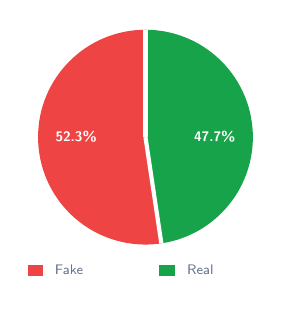
\begin{tikzpicture}[scale=.88]
      \fill[ARed](0,0)--(90:1.55cm)
        arc[start angle=90,end angle=278.5,radius=1.55cm]--cycle;
      \fill[AGreen](0,0)--(278.5:1.55cm)
        arc[start angle=278.5,end angle=450,radius=1.55cm]--cycle;
      \draw[white,line width=1.5pt](0,0)--(90:1.55cm);
      \draw[white,line width=1.5pt](0,0)--(278.5:1.55cm);
      \node[font=\tiny\bfseries,text=white] at (180:1.0cm){52.3\%};
      \node[font=\tiny\bfseries,text=white] at (0:1.0cm){47.7\%};
      \fill[ARed]  (-1.7,-2.0) rectangle ++(.22,.16);
      \node[anchor=west,font=\tiny,text=Slate] at (-1.45,-1.92){Fake};
      \fill[AGreen](0.2,-2.0) rectangle ++(.22,.16);
      \node[anchor=west,font=\tiny,text=Slate] at (0.46,-1.92){Real};
    \end{tikzpicture}
  \end{tcolorbox}
\end{column}
\begin{column}{.54\textwidth}
  \begin{tcolorbox}[mycard={BlueMid}{ABlue}]
    {\footnotesize\textbf{Key EDA Insights}}\\[3pt]
    \begin{tcolorbox}[sideline={ARed},top=1pt,bottom=1pt]
      {\tiny\textbf{\color{ARed}Near-Balanced Dataset}\quad\color{Slate}52.3\% fake --- minimal class imbalance}
    \end{tcolorbox}\vspace{1pt}
    \begin{tcolorbox}[sideline={ABlue},top=1pt,bottom=1pt]
      {\tiny\textbf{\color{ABlue}Rich Text Content}\quad\color{Slate}Articles avg 400--600 words; titles add signal}
    \end{tcolorbox}\vspace{1pt}
    \begin{tcolorbox}[sideline={AGreen},top=1pt,bottom=1pt]
      {\tiny\textbf{\color{AGreen}Subject Diversity}\quad\color{Slate}Politics, World News dominate both classes}
    \end{tcolorbox}\vspace{1pt}
    \begin{tcolorbox}[sideline={AOrange},top=1pt,bottom=1pt]
      {\tiny\textbf{\color{AOrange}Text Length Overlap}\quad\color{Slate}Similar lengths; content quality differs}
    \end{tcolorbox}\vspace{1pt}
    \begin{tcolorbox}[sideline={APurple},top=1pt,bottom=1pt]
      {\tiny\textbf{\color{APurple}Combined Title+Text}\quad\color{Slate}Merging both improves classification}
    \end{tcolorbox}
  \end{tcolorbox}
\end{column}
\end{columns}
\sfooter
\end{frame}

%------------------------------------------------------------
% SLIDE 5: PREPROCESSING PIPELINE
%------------------------------------------------------------
\begin{frame}[t]
\frametitle{03 --- Text Preprocessing Pipeline}
\framesubtitle{OOP TextPreprocessor class --- configurable, reusable, production-ready}
\vspace{.08cm}
% 6-step flow diagram
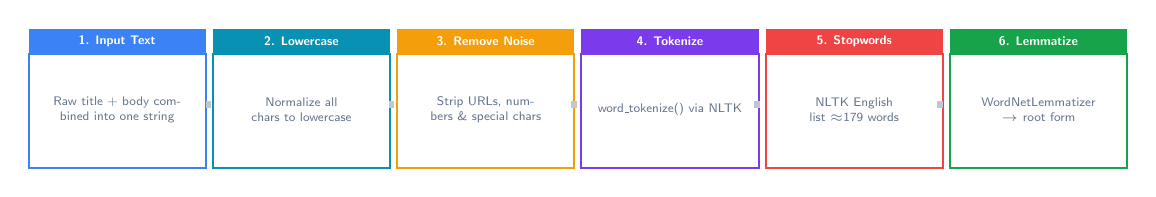
\begin{tikzpicture}[scale=0.9, transform shape]
  \pbox{ABlue}{0}{1. Input Text}{Raw title + body combined into one string}
  \pbox{ATeal}{2.6}{2. Lowercase}{Normalize all chars to lowercase}
  \pbox{AOrange}{5.2}{3. Remove Noise}{Strip URLs, numbers \& special chars}
  \pbox{APurple}{7.8}{4. Tokenize}{word\_tokenize() via NLTK}
  \pbox{ARed}{10.4}{5. Stopwords}{NLTK English list $\approx$179 words}
  \pbox{AGreen}{13.0}{6. Lemmatize}{WordNetLemmatizer $\to$ root form}
  % Arrows
  \fill[Slate!40](2.5,-.76) rectangle ++(0.08,.10);
  \fill[Slate!40](5.08,-.76) rectangle ++(0.08,.10);
  \fill[Slate!40](7.66,-.76) rectangle ++(0.08,.10);
  \fill[Slate!40](10.24,-.76) rectangle ++(0.08,.10);
  \fill[Slate!40](12.82,-.76) rectangle ++(0.08,.10);
\end{tikzpicture}

\vspace{.18cm}
\begin{columns}[T]
\begin{column}{.46\textwidth}
  \begin{tcolorbox}[codeblock,title={\textbf{CONFIG --- Preprocessing Flags}},
      colbacktitle=Navy,coltitle=ABlue,fonttitle=\scriptsize\bfseries]
    \textcolor{CodeGray}{'remove\_urls'}\ \ \ \ \ \ :\ \textcolor{AGreen}{True}\\
    \textcolor{CodeGray}{'remove\_numbers'}\ \ :\ \textcolor{AGreen}{True}\\
    \textcolor{CodeGray}{'remove\_stopwords'}:\ \textcolor{AGreen}{True}\\
    \textcolor{CodeGray}{'lemmatize'}\ \ \ \ \ \ \ :\ \textcolor{AGreen}{True}\\
    \textcolor{CodeGray}{'min\_token\_len'}\ \ \ :\ \textcolor{ABlue}{2}
  \end{tcolorbox}
\end{column}
\begin{column}{.51\textwidth}
  \begin{tcolorbox}[mycard={AGreen}{AGreen}]
    {\footnotesize\textbf{Why OOP TextPreprocessor?}}\\[3pt]
    \tikz{\fill[AGreen](0,0)circle(3pt);}\ \textbf{\textcolor{AGreen}{Reusable:}}\ %
    {\scriptsize\color{Slate}Import in any pipeline, no copy-paste}\\[2pt]
    \tikz{\fill[ABlue](0,0)circle(3pt);}\ \textbf{\textcolor{ABlue}{Configurable:}}\ %
    {\scriptsize\color{Slate}All flags via central CONFIG}\\[2pt]
    \tikz{\fill[AOrange](0,0)circle(3pt);}\ \textbf{\textcolor{AOrange}{Testable:}}\ %
    {\scriptsize\color{Slate}Unit-testable clean() method}\\[2pt]
    \tikz{\fill[APurple](0,0)circle(3pt);}\ \textbf{\textcolor{APurple}{Loggable:}}\ %
    {\scriptsize\color{Slate}Logs avg token count after transform}
  \end{tcolorbox}
\end{column}
\end{columns}
\sfooter
\end{frame}

%------------------------------------------------------------
% SLIDE 6: TF-IDF
%------------------------------------------------------------
\begin{frame}[t]
\frametitle{04 --- TF-IDF Feature Engineering}
\framesubtitle{Term Frequency--Inverse Document Frequency with bigrams}
\vspace{-0.5cm}
\begin{columns}[T]
\begin{column}{.46\textwidth}
  \begin{tcolorbox}[mycard={BlueMid}{ABlue}]
    {\footnotesize\textbf{What is TF-IDF?}}\\[3pt]
    {\scriptsize TF-IDF converts raw text to numerical vectors measuring word importance
    relative to the corpus.}\\[5pt]
    \begin{tcolorbox}[mycard={ABlue}{ABlue},colback=BlueL,top=2pt,bottom=2pt]
      \textbf{\textcolor{ABlue}{TF(t,d)}}\ {\scriptsize\color{Navy}= Count(t,d) / Total terms in d}
    \end{tcolorbox}\vspace{2pt}
    \begin{tcolorbox}[mycard={AGreen}{AGreen},colback=GreenL,top=2pt,bottom=2pt]
      \textbf{\textcolor{AGreen}{IDF(t)}}\ {\scriptsize\color{Navy}= log(Total docs / Docs with t)}
    \end{tcolorbox}\vspace{2pt}
    \begin{tcolorbox}[mycard={APurple}{APurple},colback=PurpleL,top=2pt,bottom=2pt]
      \textbf{\textcolor{APurple}{TF-IDF}}\ {\scriptsize\color{Navy}= TF(t,d) $\times$ IDF(t)}
    \end{tcolorbox}
\vspace{.06cm}
    \begin{tcolorbox}[sideline={AOrange},top=2pt,bottom=2pt]
      {\scriptsize\textit{\textbf{Why bigrams?} ``reuters confirmed'', ``fake news'' carry
      phrase-level meaning that unigrams miss.}}
    \end{tcolorbox}
  \end{tcolorbox}
\end{column}
\begin{column}{.51\textwidth}
  \begin{tcolorbox}[codeblock,title={\textbf{TfidfVectorizer Config}},
      colbacktitle=Navy,coltitle=ABlue,fonttitle=\scriptsize\bfseries]
    \textcolor{CodeGray}{max\_features}\ :\ \textcolor{ABlue}{50{,}000}\\
    \textcolor{CodeGray}{ngram\_range}\ \ :\ \textcolor{ABlue}{(1,\,2)}\ \ \ \textcolor{CodeGray}{\# bigrams}\\
    \textcolor{CodeGray}{sublinear\_tf}\ :\ \textcolor{AGreen}{True}\ \ \textcolor{CodeGray}{\# log scaling}\\
    \textcolor{CodeGray}{min\_df}\ \ \ \ \ \ \ :\ \textcolor{ABlue}{3}\ \ \ \ \ \ \textcolor{CodeGray}{\# noise filter}
  \end{tcolorbox}
  \vspace{.1cm}
  \begin{tcolorbox}[mycard={ATeal}{ATeal},title={\textbf{Train / Test Split}},
      colbacktitle=ATeal,coltitle=white,fonttitle=\small\bfseries]
    \centering
    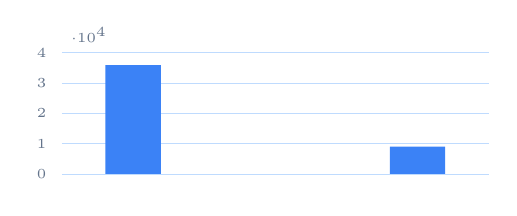
\begin{tikzpicture}
      \begin{axis}[indbar,ymin=0,ymax=42000,
        symbolic x coords={Train (80\%),Test (20\%)},
        xtick=data,width=7cm,height=3.2cm,bar width=20pt]
        \addplot[fill=ABlue,draw=none] coordinates
          {(Train (80\%),35918)(Test (20\%),8980)};
      \end{axis}
    \end{tikzpicture}
  \end{tcolorbox}
\end{column}
\end{columns}
\sfooter
\end{frame}

%------------------------------------------------------------
% SLIDE 7: MODEL TRAINING
%------------------------------------------------------------
\begin{frame}[t]
\frametitle{05 --- Model Training \& Cross-Validation}
\framesubtitle{4 classifiers trained with 5-Fold Stratified Cross-Validation}
\vspace{.04cm}
\begin{columns}[T]
\begin{column}{.245\textwidth}
  \begin{tcolorbox}[mycard={ABlue}{ABlue},top=0pt,left=0pt,right=0pt,bottom=3pt]
    \begin{tcolorbox}[statbox={ABlue},arc=0pt,top=3pt,bottom=3pt]
      {\scriptsize\bfseries\color{white}Logistic Regression}
    \end{tcolorbox}
    \vspace{2pt}\centering
    {\footnotesize\bfseries\color{ABlue}99.1\%}\,{\tiny\color{Slate}Acc}\quad
    {\footnotesize\bfseries\color{ABlue}99.1\%}\,{\tiny\color{Slate}F1}\\[1pt]
    {\footnotesize\bfseries\color{ABlue}99.8\%}\,{\tiny\color{Slate}AUC}\quad
    {\footnotesize\bfseries\color{ABlue}99.0\%}\,{\tiny\color{Slate}CV}\\
    \vspace{3pt}\hrule height .4pt\vspace{3pt}
    {\tiny\color{Slate}Fast, interpretable baseline. Coefficients reveal fake/real indicators.}
  \end{tcolorbox}
\end{column}
\begin{column}{.245\textwidth}
  \begin{tcolorbox}[mycard={APurple}{APurple},top=0pt,left=0pt,right=0pt,bottom=3pt]
    \begin{tcolorbox}[statbox={APurple},arc=0pt,top=3pt,bottom=3pt]
      {\scriptsize\bfseries\color{white}LinearSVC (Calibrated)}
    \end{tcolorbox}
    \vspace{2pt}\centering
    {\footnotesize\bfseries\color{APurple}99.3\%}\,{\tiny\color{Slate}Acc}\quad
    {\footnotesize\bfseries\color{APurple}99.3\%}\,{\tiny\color{Slate}F1}\\[1pt]
    {\footnotesize\bfseries\color{APurple}99.9\%}\,{\tiny\color{Slate}AUC}\quad
    {\footnotesize\bfseries\color{APurple}99.2\%}\,{\tiny\color{Slate}CV}\\
    \vspace{3pt}\hrule height .4pt\vspace{3pt}
    {\tiny\color{Slate}SVM with probability calibration. Best margin-maximizing for TF-IDF.}
  \end{tcolorbox}
\end{column}
\begin{column}{.245\textwidth}
  \begin{tcolorbox}[mycard={AOrange}{AOrange},top=0pt,left=0pt,right=0pt,bottom=3pt]
    \begin{tcolorbox}[statbox={AOrange},arc=0pt,top=3pt,bottom=3pt]
      {\scriptsize\bfseries\color{white}Naive Bayes (MNB)}
    \end{tcolorbox}
    \vspace{2pt}\centering
    {\footnotesize\bfseries\color{AOrange}95.8\%}\,{\tiny\color{Slate}Acc}\quad
    {\footnotesize\bfseries\color{AOrange}95.7\%}\,{\tiny\color{Slate}F1}\\[1pt]
    {\footnotesize\bfseries\color{AOrange}99.2\%}\,{\tiny\color{Slate}AUC}\quad
    {\footnotesize\bfseries\color{AOrange}95.6\%}\,{\tiny\color{Slate}CV}\\
    \vspace{3pt}\hrule height .4pt\vspace{3pt}
    {\tiny\color{Slate}Probabilistic, fast. Excellent AUC. Assumes term independence.}
  \end{tcolorbox}
\end{column}
\begin{column}{.245\textwidth}
  \begin{tcolorbox}[mycard={AGreen}{AGreen},top=0pt,left=0pt,right=0pt,bottom=3pt]
    \begin{tcolorbox}[statbox={AGreen},arc=0pt,top=3pt,bottom=3pt]
      {\scriptsize\bfseries\color{white}Random Forest}
    \end{tcolorbox}
    \vspace{2pt}\centering
    {\footnotesize\bfseries\color{AGreen}98.6\%}\,{\tiny\color{Slate}Acc}\quad
    {\footnotesize\bfseries\color{AGreen}98.5\%}\,{\tiny\color{Slate}F1}\\[1pt]
    {\footnotesize\bfseries\color{AGreen}99.7\%}\,{\tiny\color{Slate}AUC}\quad
    {\footnotesize\bfseries\color{AGreen}98.4\%}\,{\tiny\color{Slate}CV}\\
    \vspace{3pt}\hrule height .4pt\vspace{3pt}
    {\tiny\color{Slate}100 decision trees. Robust to overfitting; captures non-linear interactions.}
  \end{tcolorbox}
\end{column}
\end{columns}
\vspace{.08cm}
\begin{tcolorbox}[sideline={ABlue},top=2pt,bottom=2pt]
  {\scriptsize\textit{\textbf{5-Fold Stratified CV} ensures results generalise ---
  not a fluke of one split. \texttt{stratify=True} maintains class ratios in every fold.}}
\end{tcolorbox}
\vspace{.06cm}
\begin{tcolorbox}[mycard={BlueMid}{ABlue},colback=BlueL,top=2pt,bottom=2pt]
\centering
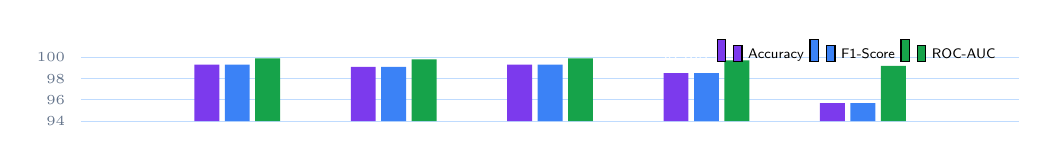
\begin{tikzpicture}
  \begin{axis}[indbar,ymin=94,ymax=100.8,
    symbolic x coords={LinearSVC,LogReg,Ensemble,Rnd Forest,Naive Bayes},
    xtick=data,width=13.5cm,height=2.5cm,bar width=9pt,
    legend style={at={(.99,1.22)},anchor=north east,font=\tiny,draw=none,
      fill=none,legend columns=3}]
    \addplot[fill=APurple,draw=none] coordinates
      {(LinearSVC,99.3)(LogReg,99.1)(Ensemble,99.3)(Rnd Forest,98.5)(Naive Bayes,95.7)};
    \addplot[fill=ABlue,draw=none] coordinates
      {(LinearSVC,99.3)(LogReg,99.1)(Ensemble,99.3)(Rnd Forest,98.5)(Naive Bayes,95.7)};
    \addplot[fill=AGreen,draw=none] coordinates
      {(LinearSVC,99.9)(LogReg,99.8)(Ensemble,99.9)(Rnd Forest,99.7)(Naive Bayes,99.2)};
    \legend{Accuracy,F1-Score,ROC-AUC}
  \end{axis}
\end{tikzpicture}
\end{tcolorbox}
\sfooter
\end{frame}

%------------------------------------------------------------
% SLIDE 8: ENSEMBLE
%------------------------------------------------------------
\begin{frame}[t]
\frametitle{06 --- Ensemble Voting Classifier}
\framesubtitle{Soft Voting --- combining Logistic Regression + LinearSVC + Naive Bayes}
\vspace{.1cm}
\begin{columns}[T]
\begin{column}{.60\textwidth}
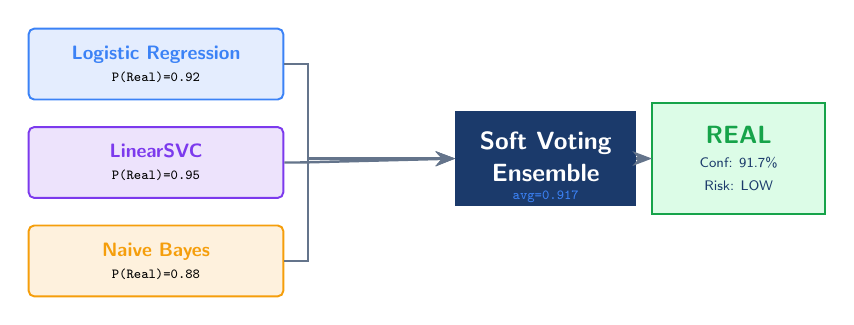
\begin{tikzpicture}[arr/.style={-Stealth,line width=.9pt,color=Slate}]
  \node[rectangle,rounded corners=2pt,draw=ABlue,fill=ABlue!14!white,
    line width=.7pt,minimum width=3.2cm,minimum height=.9cm,
    text width=3.0cm,align=center,font=\scriptsize] (lr) at (0,2.1)
    {\textbf{\color{ABlue}Logistic Regression}\\{\tiny\ttfamily P(Real)=0.92}};
  \node[rectangle,rounded corners=2pt,draw=APurple,fill=APurple!14!white,
    line width=.7pt,minimum width=3.2cm,minimum height=.9cm,
    text width=3.0cm,align=center,font=\scriptsize] (svm) at (0,0.85)
    {\textbf{\color{APurple}LinearSVC}\\{\tiny\ttfamily P(Real)=0.95}};
  \node[rectangle,rounded corners=2pt,draw=AOrange,fill=AOrange!14!white,
    line width=.7pt,minimum width=3.2cm,minimum height=.9cm,
    text width=3.0cm,align=center,font=\scriptsize] (nb) at (0,-0.4)
    {\textbf{\color{AOrange}Naive Bayes}\\{\tiny\ttfamily P(Real)=0.88}};
  \fill[Navy](3.8,0.3) rectangle ++(2.3,1.2);
  \node[font=\small\bfseries,text=white] at (4.95,1.10){Soft Voting};
  \node[font=\small\bfseries,text=white] at (4.95,0.72){Ensemble};
  \node[font=\tiny,text=ABlue]           at (4.95,0.42){\ttfamily avg=0.917};
  \draw[arr](lr.east)  -- ++(0.3,0) |- (3.8,0.9);
  \draw[arr](svm.east) -- ++(0.2,0) -- (3.8,0.9);
  \draw[arr](nb.east)  -- ++(0.3,0) |- (3.8,0.9);
  \fill[GreenL](6.3,0.2) rectangle ++(2.2,1.4);
  \draw[AGreen,line width=.7pt](6.3,0.2) rectangle ++(2.2,1.4);
  \node[font=\small\bfseries,text=AGreen] at (7.4,1.20){REAL};
  \node[font=\tiny,text=Navy]             at (7.4,0.85){Conf: 91.7\%};
  \node[font=\tiny,text=Navy]             at (7.4,0.55){Risk: LOW};
  \draw[arr](6.1,0.9)--(6.3,0.9);
\end{tikzpicture}
\end{column}
\begin{column}{.38\textwidth}
  \begin{tcolorbox}[sideline={ABlue},top=3pt,bottom=3pt]
    {\footnotesize\textbf{\color{ABlue}Variance Reduction}}\\
    {\tiny\color{Slate}Averaging predictions reduces impact of any single model's errors.}
  \end{tcolorbox}
\vspace{.06cm}
  \begin{tcolorbox}[sideline={AGreen},top=3pt,bottom=3pt]
    {\footnotesize\textbf{\color{AGreen}Robustness}}\\
    {\tiny\color{Slate}Even if one model errs, the majority vote corrects the final prediction.}
  \end{tcolorbox}
\vspace{.06cm}
  \begin{tcolorbox}[sideline={APurple},top=3pt,bottom=3pt]
    {\footnotesize\textbf{\color{APurple}Soft Voting}}\\
    {\tiny\color{Slate}Uses probability averages not hard votes --- captures confidence, not direction.}
  \end{tcolorbox}
\end{column}
\end{columns}
\sfooter
\end{frame}

%------------------------------------------------------------
% SLIDE 9: EVALUATION DASHBOARD
%------------------------------------------------------------
\begin{frame}[t]
\frametitle{07 --- Evaluation Dashboard}
\framesubtitle{Accuracy, F1-Score, ROC-AUC, Precision-Recall}
\vspace{.04cm}
\renewcommand{\arraystretch}{1.12}
{\footnotesize
\begin{tabularx}{\textwidth}{%
  >{\bfseries\color{Navy}}p{3.4cm}
  >{\centering\arraybackslash}X>{\centering\arraybackslash}X
  >{\centering\arraybackslash}X>{\centering\arraybackslash}X}
\rowcolor{Navy}
\textcolor{white}{\textbf{Model}}&\textcolor{white}{\textbf{Accuracy}}&
\textcolor{white}{\textbf{F1-Score}}&\textcolor{white}{\textbf{ROC-AUC}}&
\textcolor{white}{\textbf{CV F1 (mean$\pm$std)}}\\
\rowcolor{GreenL}
\textbf{LinearSVC (Calibrated)}&\textcolor{AGreen}{\textbf{99.3\%}}&
\textcolor{AGreen}{\textbf{99.3\%}}&\textcolor{AGreen}{\textbf{99.9\%}}&
\textcolor{AGreen}{\textbf{99.2\% $\pm$ 0.1\%}}\\
Logistic Regression&99.1\%&99.1\%&99.8\%&99.0\% $\pm$ 0.1\%\\
\rowcolor{GreenL}
\textbf{Ensemble (Voting)}&\textcolor{AGreen}{\textbf{99.3\%}}&
\textcolor{AGreen}{\textbf{99.3\%}}&\textcolor{AGreen}{\textbf{99.9\%}}&---\\
Random Forest&98.6\%&98.5\%&99.7\%&98.4\% $\pm$ 0.2\%\\
\rowcolor{SlateL}
Naive Bayes&95.8\%&95.7\%&99.2\%&95.6\% $\pm$ 0.3\%\\
\end{tabularx}}
\vspace{.1cm}
\begin{columns}[T]
\begin{column}{.49\textwidth}
  \begin{tcolorbox}[mycard={BlueMid}{ABlue},top=2pt,bottom=2pt]
    \centering{\footnotesize\textbf{ROC-AUC by Model (\%)}}\\[2pt]
    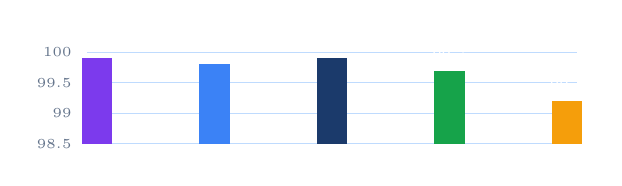
\begin{tikzpicture}
      \begin{axis}[indbar,ymin=98.5,ymax=100.2,
        symbolic x coords={LinearSVC,LogReg,Ensemble,Rnd Forest,Naive Bayes},
        xtick=data,width=7.8cm,height=2.9cm,bar width=11pt]
        \addplot[fill=APurple,draw=none] coordinates {(LinearSVC,99.9)};
        \addplot[fill=ABlue,  draw=none] coordinates {(LogReg,99.8)};
        \addplot[fill=Navy,   draw=none] coordinates {(Ensemble,99.9)};
        \addplot[fill=AGreen, draw=none] coordinates {(Rnd Forest,99.7)};
        \addplot[fill=AOrange,draw=none] coordinates {(Naive Bayes,99.2)};
      \end{axis}
    \end{tikzpicture}
  \end{tcolorbox}
\end{column}
\begin{column}{.49\textwidth}
  \begin{tcolorbox}[mycard={BlueMid}{ABlue},top=2pt,bottom=2pt]
    \centering{\footnotesize\textbf{F1-Score by Model (\%)}}\\[2pt]
    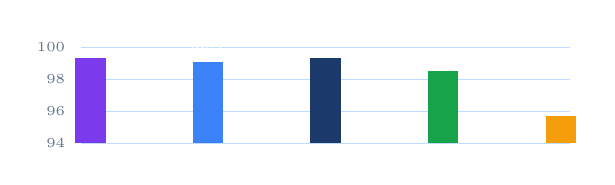
\begin{tikzpicture}
      \begin{axis}[indbar,ymin=94,ymax=100.5,
        symbolic x coords={LinearSVC,LogReg,Ensemble,Rnd Forest,Naive Bayes},
        xtick=data,width=7.8cm,height=2.9cm,bar width=11pt]
        \addplot[fill=APurple,draw=none] coordinates {(LinearSVC,99.3)};
        \addplot[fill=ABlue,  draw=none] coordinates {(LogReg,99.1)};
        \addplot[fill=Navy,   draw=none] coordinates {(Ensemble,99.3)};
        \addplot[fill=AGreen, draw=none] coordinates {(Rnd Forest,98.5)};
        \addplot[fill=AOrange,draw=none] coordinates {(Naive Bayes,95.7)};
      \end{axis}
    \end{tikzpicture}
  \end{tcolorbox}
\end{column}
\end{columns}
\sfooter
\end{frame}

%------------------------------------------------------------
% SLIDE 10: EXPLAINABILITY
%------------------------------------------------------------
\begin{frame}[t]
\frametitle{08 --- Model Explainability \& Word Clouds}
\framesubtitle{Feature importance via LR coefficients + visual term analysis}
\vspace{.04cm}
\begin{columns}[T]
\begin{column}{.49\textwidth}
  \begin{tcolorbox}[mycard={ARed}{ARed},top=2pt,bottom=2pt]
    \centering{\footnotesize\textbf{\color{ARed}Top Fake News Indicators}}\\[2pt]
    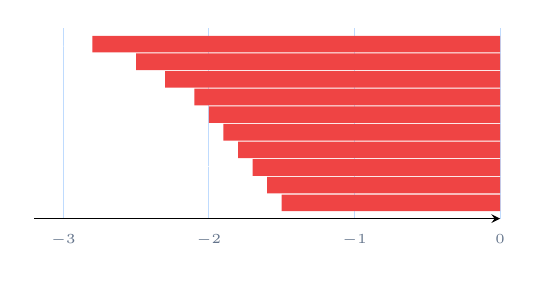
\begin{tikzpicture}
      \begin{axis}[xbar,bar width=6pt,xmin=-3.2,xmax=0,ytick=data,
        yticklabels={liberal,exposed,conspiracy,share,via,watch,video,obama,hillary,trump},
        yticklabel style={font=\tiny,color=Slate},
        x tick label style={font=\tiny,color=Slate},
        xmajorgrids,grid style={color=BlueMid},
        axis y line=none,axis x line=bottom,tick style={draw=none},
        width=7.5cm,height=4.0cm,
        nodes near coords,
        every node near coord/.style={font=\tiny,color=white,xshift=-2pt},clip=false]
        \addplot[fill=ARed,draw=none] coordinates
          {(-1.5,0)(-1.6,1)(-1.7,2)(-1.8,3)(-1.9,4)
           (-2.0,5)(-2.1,6)(-2.3,7)(-2.5,8)(-2.8,9)};
      \end{axis}
    \end{tikzpicture}
  \end{tcolorbox}
\end{column}
\begin{column}{.49\textwidth}
  \begin{tcolorbox}[mycard={AGreen}{AGreen},top=2pt,bottom=2pt]
    \centering{\footnotesize\textbf{\color{AGreen}Top Real News Indicators}}\\[2pt]
    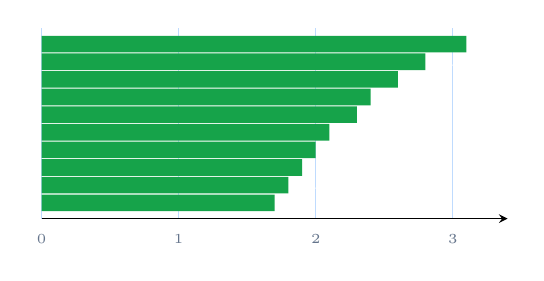
\begin{tikzpicture}
      \begin{axis}[xbar,bar width=6pt,xmin=0,xmax=3.4,ytick=data,
        yticklabels={government,reported,percent,minister,confirmed,official,according,statement,said,reuters},
        yticklabel style={font=\tiny,color=Slate},
        x tick label style={font=\tiny,color=Slate},
        xmajorgrids,grid style={color=BlueMid},
        axis y line=none,axis x line=bottom,tick style={draw=none},
        width=7.5cm,height=4.0cm,
        nodes near coords,
        every node near coord/.style={font=\tiny,color=white,xshift=2pt},clip=false]
        \addplot[fill=AGreen,draw=none] coordinates
          {(1.7,0)(1.8,1)(1.9,2)(2.0,3)(2.1,4)
           (2.3,5)(2.4,6)(2.6,7)(2.8,8)(3.1,9)};
      \end{axis}
    \end{tikzpicture}
  \end{tcolorbox}
\end{column}
\end{columns}
\vspace{.06cm}
\begin{columns}[T]
\begin{column}{.32\textwidth}
  \begin{tcolorbox}[sideline={ARed},top=3pt,bottom=3pt]
    {\footnotesize\textbf{\color{ARed}Fake News Language}}\\
    {\tiny\color{Slate}Political names, emotional verbs, social sharing cues and unverified claims.}
  \end{tcolorbox}
\end{column}
\begin{column}{.32\textwidth}
  \begin{tcolorbox}[sideline={AGreen},top=3pt,bottom=3pt]
    {\footnotesize\textbf{\color{AGreen}Real News Language}}\\
    {\tiny\color{Slate}Sources (``reuters''), attribution (``confirmed'', ``said''), official roles and data.}
  \end{tcolorbox}
\end{column}
\begin{column}{.32\textwidth}
  \begin{tcolorbox}[sideline={ABlue},top=3pt,bottom=3pt]
    {\footnotesize\textbf{\color{ABlue}Key Takeaway}}\\
    {\tiny\color{Slate}The model learns \emph{style}, not just topic. Real news uses sourced, attributed language.}
  \end{tcolorbox}
\end{column}
\end{columns}
\sfooter
\end{frame}

%------------------------------------------------------------
% SLIDE 11: PRODUCTION DEPLOYMENT
%------------------------------------------------------------
\begin{frame}[t]
\frametitle{09 --- Production Deployment}
\framesubtitle{Model persistence, reload verification, inference with confidence scoring}
\vspace{.06cm}
\begin{columns}[T]
\begin{column}{.44\textwidth}
  \begin{tcolorbox}[mycard={BlueMid}{ABlue},title={\footnotesize\textbf{Model Persistence (joblib)}},
      colbacktitle=ABlue,coltitle=white]
    \tikz{\fill[ABlue](0,0)circle(4pt);}\ \textbf{\textcolor{ABlue}{1. Train}}\ %
    {\scriptsize\color{Slate}Fit TF-IDF + best classifier on training set}\\[4pt]
    \tikz{\fill[APurple](0,0)circle(4pt);}\ \textbf{\textcolor{APurple}{2. Save}}\ %
    {\scriptsize\color{Slate}joblib.dump(model) + joblib.dump(tfidf)}\\[4pt]
    \tikz{\fill[AGreen](0,0)circle(4pt);}\ \textbf{\textcolor{AGreen}{3. Verify}}\ %
    {\scriptsize\color{Slate}Reload + re-predict --- assert predictions match}\\[4pt]
    \tikz{\fill[AOrange](0,0)circle(4pt);}\ \textbf{\textcolor{AOrange}{4. Deploy}}\ %
    {\scriptsize\color{Slate}Load once at startup; serve many requests}
  \end{tcolorbox}
\end{column}
\begin{column}{.54\textwidth}
  \begin{tcolorbox}[codeblock,title={\textbf{predict\_article() Function}},
      colbacktitle=Navy,coltitle=ABlue,fonttitle=\scriptsize\bfseries]
    \textcolor{ABlue}{def} \textcolor{white}{predict\_article(text, threshold=0.5):}\\
    \ \ \textcolor{CodeGray}{clean}\ =\ preprocessor.clean(text)\\
    \ \ \textcolor{CodeGray}{vec}\ \ \ =\ tfidf.transform([clean])\\
    \ \ \textcolor{CodeGray}{proba}\ =\ model.predict\_proba(vec)[0][1]\\
    \ \ \textcolor{CodeGray}{conf}\ \ =\ proba\ \textcolor{ABlue}{if}\ pred==1\ \textcolor{ABlue}{else}\ (1-proba)\\
    \ \ \textcolor{CodeGray}{risk}\ \ =\ \textcolor{AGreen}{'LOW'}\ \ \textcolor{ABlue}{if}\ conf>0.90\\
    \ \ \ \ \ \ \ \ \ \ \ \textcolor{AGreen}{'MEDIUM'}\ \textcolor{ABlue}{if}\ conf>0.70\\
    \ \ \ \ \ \ \ \ \ \ \ \textcolor{AGreen}{else\ 'HIGH'}\\
    \ \ \textcolor{ABlue}{return}\ \{\\
    \ \ \ \ \textcolor{AGreen}{'prediction'}:\ 'REAL'\ or\ 'FAKE',\\
    \ \ \ \ \textcolor{AGreen}{'confidence'}:\ conf\ *\ 100,\\
    \ \ \ \ \textcolor{AGreen}{'risk\_level'}:\ risk\ \}
  \end{tcolorbox}
\end{column}
\end{columns}
\vspace{.08cm}
\begin{columns}[T]
\begin{column}{.32\textwidth}
  \begin{tcolorbox}[mycard={AGreen}{AGreen},colback=GreenL,top=2pt,bottom=2pt]
    \centering{\small\bfseries\color{AGreen}REAL}\ %
    {\scriptsize Conf:~95.2\%\ Risk:~LOW}
  \end{tcolorbox}
\end{column}
\begin{column}{.32\textwidth}
  \begin{tcolorbox}[mycard={ARed}{ARed},colback=RedL,top=2pt,bottom=2pt]
    \centering{\small\bfseries\color{ARed}FAKE}\ %
    {\scriptsize Conf:~97.8\%\ Risk:~LOW}
  \end{tcolorbox}
\end{column}
\begin{column}{.32\textwidth}
  \begin{tcolorbox}[mycard={AOrange}{AOrange},colback=OrangeL,top=2pt,bottom=2pt]
    \centering{\small\bfseries\color{AOrange}FAKE}\ %
    {\scriptsize Conf:~71.3\%\ Risk:~MEDIUM}
  \end{tcolorbox}
\end{column}
\end{columns}
\sfooter
\end{frame}

%------------------------------------------------------------
% SLIDE 12: RESULTS & TAKEAWAYS
%------------------------------------------------------------
\begin{frame}[t]
\frametitle{10 --- Results \& Key Takeaways}
\framesubtitle{Industrial-grade fake news detection --- project summary}
\vspace{.06cm}
\begin{columns}[T]
\begin{column}{.24\textwidth}
  \begin{tcolorbox}[statbox={BlueL},colframe=ABlue]
    {\Large\bfseries\color{ABlue}$\sim$99\%}\\[2pt]{\tiny\color{ABlue}Best Accuracy}
  \end{tcolorbox}
\end{column}
\begin{column}{.24\textwidth}
  \begin{tcolorbox}[statbox={GreenL},colframe=AGreen]
    {\Large\bfseries\color{AGreen}$\sim$99\%}\\[2pt]{\tiny\color{AGreen}Best F1-Score}
  \end{tcolorbox}
\end{column}
\begin{column}{.24\textwidth}
  \begin{tcolorbox}[statbox={PurpleL},colframe=APurple]
    {\Large\bfseries\color{APurple}$\sim$99.9\%}\\[2pt]{\tiny\color{APurple}ROC-AUC Score}
  \end{tcolorbox}
\end{column}
\begin{column}{.24\textwidth}
  \begin{tcolorbox}[statbox={OrangeL},colframe=AOrange]
    {\Large\bfseries\color{AOrange}44,898}\\[2pt]{\tiny\color{AOrange}Articles Trained}
  \end{tcolorbox}
\end{column}
\end{columns}
\vspace{.1cm}
\begin{columns}[T]
\begin{column}{.46\textwidth}
  \begin{tcolorbox}[mycard={BlueMid}{ABlue},title={\footnotesize\textbf{Industrial Additions}},
      colbacktitle=NavyML,coltitle=white]
    \scriptsize
    \tikz{\fill[ABlue](0,0)circle(2.5pt);}\ Central CONFIG object\\[1pt]
    \tikz{\fill[ATeal](0,0)circle(2.5pt);}\ Python logging + timestamps\\[1pt]
    \tikz{\fill[AGreen](0,0)circle(2.5pt);}\ OOP TextPreprocessor --- reusable class\\[1pt]
    \tikz{\fill[APurple](0,0)circle(2.5pt);}\ 4 models + Soft Voting Ensemble\\[1pt]
    \tikz{\fill[AOrange](0,0)circle(2.5pt);}\ 5-Fold Cross-Validation\\[1pt]
    \tikz{\fill[ARed](0,0)circle(2.5pt);}\ ROC-AUC + Precision-Recall curves\\[1pt]
    \tikz{\fill[ABlue](0,0)circle(2.5pt);}\ Feature importance --- explainable AI\\[1pt]
    \tikz{\fill[AGreen](0,0)circle(2.5pt);}\ joblib save/load + reload verify\\[1pt]
    \tikz{\fill[ATeal](0,0)circle(2.5pt);}\ Inference with confidence \& risk level
  \end{tcolorbox}
\end{column}
\begin{column}{.51\textwidth}
  \begin{tcolorbox}[mycard={ATeal}{ATeal},title={\footnotesize\textbf{Key Learnings}},
      colbacktitle=ATeal,coltitle=white]
    \begin{tcolorbox}[sideline={ABlue},top=2pt,bottom=2pt]
      {\footnotesize\textbf{\color{ABlue}99\% Accuracy $\neq$ Done}}\\
      {\tiny\color{Slate}Production means explainability, persistence \& structured inference.}
    \end{tcolorbox}\vspace{2pt}
    \begin{tcolorbox}[sideline={AGreen},top=2pt,bottom=2pt]
      {\footnotesize\textbf{\color{AGreen}Bigrams Add Value}}\\
      {\tiny\color{Slate}Phrases like ``reuters said'' dramatically improve signal vs.\ unigrams.}
    \end{tcolorbox}\vspace{2pt}
    \begin{tcolorbox}[sideline={AOrange},top=2pt,bottom=2pt]
      {\footnotesize\textbf{\color{AOrange}Ensemble $>$ Single}}\\
      {\tiny\color{Slate}Soft voting reduces variance; catches errors missed by any one model.}
    \end{tcolorbox}\vspace{2pt}
    \begin{tcolorbox}[sideline={APurple},top=2pt,bottom=2pt]
      {\footnotesize\textbf{\color{APurple}Config-Driven Code}}\\
      {\tiny\color{Slate}Centralising hyperparameters makes experiments reproducible.}
    \end{tcolorbox}
  \end{tcolorbox}
\end{column}
\end{columns}
\begin{tikzpicture}[remember picture,overlay]
  \fill[Navy]
    ([yshift=.33cm]current page.south west) rectangle ++(\paperwidth,.45cm);
  \node[font=\small\bfseries,text=white,anchor=center] at
    ([yshift=.55cm]current page.south)
    {Completed as part of Elevvo Internship Program\ \textbullet\
     Task 3: Fake News Detection\ \textbullet\ Abdullah Zahid};
\end{tikzpicture}
\end{frame}

%------------------------------------------------------------
% SLIDE 13: CLOSING
%------------------------------------------------------------
{\setbeamercolor{background canvas}{bg=NavyDark}
\begin{frame}[plain]
\begin{tikzpicture}[remember picture,overlay]
  \fill[NavyML,opacity=.32]
    ([xshift=2cm,yshift=-3cm]current page.south east) circle(3cm);
  \fill[ABlue,opacity=.16]
    ([xshift=-1.5cm,yshift=1.5cm]current page.north west) circle(2.2cm);
  \fill[ABlue](current page.north west) rectangle ++(.11,-\paperheight);
  \node[anchor=north west,
    font=\fontsize{40}{44}\bfseries\selectfont,text=white] at
    ([xshift=.55cm,yshift=-1.4cm]current page.north west){Thank You};
  \node[anchor=north west,font=\large\itshape,text=ABlue,text width=12cm] at
    ([xshift=.55cm,yshift=-2.9cm]current page.north west)
    {Fake News Detection --- Industrial Grade NLP Pipeline};
  \draw[ABlue,line width=1.5pt]
    ([xshift=.55cm,yshift=-3.52cm]current page.north west) -- ++(6.5cm,0);
  \node[anchor=north west,font=\small,text=Slate,text width=7cm] at
    ([xshift=.55cm,yshift=-3.75cm]current page.north west)
    {Abdullah Zahid\\[4pt]
     Elevvo Internship Program\\[4pt]
     Task 3 --- NLP Binary Classification};
  % Tech stack tiles
  \fill[NavyMid]
    ([xshift=7.4cm,yshift=-3.55cm]current page.north west) rectangle ++(2.3cm,.54cm);
  \node[font=\scriptsize,text=ABlue] at
    ([xshift=8.55cm,yshift=-3.28cm]current page.north west){Python};
  \fill[NavyMid]
    ([xshift=10.1cm,yshift=-3.55cm]current page.north west) rectangle ++(2.3cm,.54cm);
  \node[font=\scriptsize,text=ABlue] at
    ([xshift=11.25cm,yshift=-3.28cm]current page.north west){NLTK / spaCy};
  \fill[NavyMid]
    ([xshift=12.8cm,yshift=-3.55cm]current page.north west) rectangle ++(2.3cm,.54cm);
  \node[font=\scriptsize,text=ABlue] at
    ([xshift=13.95cm,yshift=-3.28cm]current page.north west){Scikit-learn};
  \fill[NavyMid]
    ([xshift=7.4cm,yshift=-4.55cm]current page.north west) rectangle ++(2.3cm,.54cm);
  \node[font=\scriptsize,text=ABlue] at
    ([xshift=8.55cm,yshift=-4.28cm]current page.north west){TF-IDF};
  \fill[NavyMid]
    ([xshift=10.1cm,yshift=-4.55cm]current page.north west) rectangle ++(2.3cm,.54cm);
  \node[font=\scriptsize,text=ABlue] at
    ([xshift=11.25cm,yshift=-4.28cm]current page.north west){Ensemble ML};
  \fill[NavyMid]
    ([xshift=12.8cm,yshift=-4.55cm]current page.north west) rectangle ++(2.3cm,.54cm);
  \node[font=\scriptsize,text=ABlue] at
    ([xshift=13.95cm,yshift=-4.28cm]current page.north west){joblib};
  \fill[NavyMid](current page.south west) rectangle ++(\paperwidth,.38cm);
  \node[anchor=center,font=\tiny,text=Slate] at
    ([yshift=.19cm]current page.south)
    {Elevvo Internship Program\ \textbullet\
     Fake News Detection\ \textbullet\ NLP \& ML};
\end{tikzpicture}
\end{frame}}

\end{document}